\documentclass{article}

\usepackage[brazil]{babel}
\usepackage[utf8]{inputenc}
\usepackage[T1]{fontenc}% optional T1 font encoding
\usepackage[%
    colorlinks=true,
    pdfborder={0 0 0},
    linkcolor=red
]{hyperref}
\usepackage[all]{hypcap}
\usepackage{amsmath}
\interdisplaylinepenalty=2500
\usepackage{graphicx}
\usepackage[cmintegrals]{newtxmath}
\usepackage{cite}
\usepackage{listings}
\usepackage{hyperref}
\usepackage{indentfirst}
\usepackage{siunitx}
\usepackage{textgreek}
\usepackage[portuguese,linesnumbered,ruled]{algorithm2e}
\usepackage{multirow}
\usepackage{anysize}

\begin{document}

\title{ Filtros com Constante de Tempo Simples (CTS) e familiarização com os instrumentos de bancada}
\author{Bianca Yoshie Itiroko - 164923, Luiz Eduardo Cartolano - 183012, \\ Seong Kim - 177143 \\ EE534 - Turma Y - Grupo 2}
\date{Agosto de 2018}

\maketitle

\begin{abstract}
    A primeira parte do experimento consiste na familiarização com os equipamentos e no estudo do método de medida com o \emph{cursor} e com o recurso \emph{measure} do osciloscópio, sendo que o segundo se mostrou mais preciso. A segunda parte trata-se do estudo de circuitos passa baixa e passa alta quando submetidos a diferentes frequências. Analisando o diagrama de Bode obtido dos dados gerados por essa parte do experimento, pode-se ver que para circuitos passa baixa há atenuação de frequências altas. Já para circuitos passa alta há atenuação de frequências baixas, como esperado.
\end{abstract}

\section{Introdução}
Os filtros de frequência são bem comuns na eletrônica, utilizados para moldar sinais elétricos e promover a atenuação de interferências em ondas de áudio, vídeo e dados com base em suas frequências de oscilação. Um dos exemplos mais imediatos da aplicação de filtros é o equalizador de som, que permite ao usuário selecionar a atenuação desejada  do áudio em diversas faixas de frequência, e assim deixar o som conforme sua preferência. Existem dois principais tipos de filtros de frequência: os ativos e os passivos.

Neste experimento, será estudado o comportamento de filtros de frequência passivos, isso é, filtros que são compostos apenas por resistores e capacitores, sem a presença de amplificadores operacionais. Busca-se compreender as relações entre a amplitude senoidal da tensão de saída em comparação com a de entrada e as defasagens causadas pelos elementos reativos dos circuitos passa-baixa e passa-alta, em suas várias configurações. Para melhor visualização, são confeccionados diagramas de Bode dos resultados obtidos.

O experimento também buscou familiarizar os alunos com os equipamentos usados no laboratório, como o osciloscópio, gerador de ondas/funções, placa de contatos, cabos com plugs banana e coaxial, multímetro digital, resistorese capacitores.

\section{Procedimentos}
Para a realização dos experimentos propostos, foram utilizados os seguintes componentes e ferramentas: Osciloscópio digital de dois canais, gerador de ondas/funções, cabos com plugs banana e coaxial, multímetro digital, placa de contatos, capacitores de 100pF e resistores de 100k\textOmega.

A primeira parte do experimento consiste na familiariazação com os equipamentos do laboratório. Para isso conectou-se o sinal de \emph{output} do gerador de ondas/funções em um dos canais do osciloscópio digital, e usou-se os recursos \emph{cursor} e \emph{measure} deste. Nesta parte do experimento é preciso tomar cuidado com a impedância explicitada no gerador de ondas/funções que deve ser configurada para \emph{high impedance}.

A segunda parte do experimento consiste no estudo de filtros passa-alta e passa-baixa formados por um resistor e um elemento reativo em série, um capacitor. Na qual se montou um filtro como o mostrado na Figura \ref{fig:montagem}. Um detalhe importante na montagem do circuito é o uso do \emph{T(BNC)} a fim de conectar o sinal emitido pelo gerador em dois locais, a placa de contatos e um dos canais do osciloscópio.

O ponto central, denominado de V1 para esse experimento, entre o resistor e o capacitor, é o ponto de medição da tensão do gerador de ondas, e "a" e "b", denominado de V2, são os pontos de leitura da tensão filtrada por frequências (passa-baixa e passa-alta, respectivamente), ou seja, é o ponto de onde o sinal seguiria seu caminho pelos demais circuitos do componente eletrônico após ser filtrado. Para estudo das efetividade dos circuitos montados em moderar a frequência, deve-se variar a frequência do gerador de ondas senoidais em uma ampla gama, incluindo as frequências dos sinais que deseja-se atenuar ou manter. 

Para avaliar a atenuação, deve-se comparar as amplitudes de tensão  das ondas senoidais medidas em V2 (tensão de saída) com as medidas em V1 (tensão de entrada).

Ao final da segunda parte, desconectou-se o cabo BNC do canal-1, colocou-se frequência 16kHz e com duas pontas de prova efetuou-se a medida de tensão diferencial entre os nós [A] e [B].

\section{Discussão}
Na primeira parte do experimento, mediu-se a amplitude com os cursores no osciloscópio e obteve-se 5.04V e -5.12V, o que é condizente com os 10Vpp setados no gerador.
Como período, encontrou-se -508us e -404us para os extremos da função, o que nos resulta 104us, também condizente com o esperado quando calculou-se o período com a frequência setada no gerador. 
De tempos de subida e descida, obteve-se 38us para ambos.

Ainda nessa primeira parte, utilizou-se também o recurso \emph{measure} do osciloscópio. Ao analisar os dados obtidos, pode-se perceber que os mesmos são mais precisos do que os setados via cursores anteriormente: para a amplitude obteve-se 10V, para o período obteve-se 100us e nos tempos de subida e descida obteve-se 43us, que são exatamente o que foi introduzido no gerador.

Essa diferença pode ser justificada por conta de o primeiro método necessitar de ajuste humano para definir os cursores, o que provavelmente foi o que trouxe as diferenças entre os resultados.

A fim de obter comparações, configurou-se o canal para medida CA e então para medida CC. Obteve-se que para medidas em CA, ao alterar o \emph{offset}, nada variava. Já em CC, alterar o \emph{offset}, trazia deslocamentos no eixo y. Isso se deve pois quando se coloca o osciloscópio para medir CA, ele automaticamente corrige o \emph{offset}. Já quando a medida é CC, o \emph{offset}, por ser importante, não é anulado.

Para a segunda parte do experimento, montou-se o circuito da Figura  \ref{fig:montagem} em que a esquerda tem-se um filtro Passa-Baixas de primeira ordem e o circuito à direita da fonte é um filtro Passa-Altas. Com o auxílio de uma ponta de prova, realizou-se medições de diferentes frequências,  de comparar os resultados com frequências próximas ou não da frequência de corte. Os valores obtidos podem ser observados na Tabela \ref{tabela:frequencias}.

Para refinar a análise, calculou-se a frequência de corte teórica usando a Fórmula \ref{eq:corte} e obteve-se o valor de 15915 Hz, o que foi condizente com os intervalos de frequência obtidos na tabela.

\begin{equation}
    \omega_{c} = \frac{1}{RC}
    \label{eq:corte}
\end{equation}

A partir da atenuação e da fase obtidas a partir do logarítmico da frequência, utilizou-se um script em \emph{Python3} para plotar os dados e obter um diagrama de Bode. Para o circuito Passa Alta, pode-se ver que claramente existe uma atenuação maior para frequências baixas. O comportamento é fruto do fato de que o circuito é constituído por um circuito CR série, no qual a tensão de saída é a do resistor. O comportamento dele é o inverso de um filtro passa-baixa: para frequências altas a reatância capacitiva assume valores baixos em comparação ao valor da resistência, de modo que tensão de saída é praticamente igual à tensão de entrada. Para frequências baixas, a reatância capacitiva assume valores altos em comparação com o valor da resistência, atenuando a tensão de saída para um valor praticamente nulo. Como pode ser observado nas Figuras \ref{fig:passa_alta_atenuacao} e \ref{fig:passa_alta_fase}.

Da mesma forma, no circuito Passa Baixa houve atenuação mais expressiva para frequências altas, o que acontece pois o filtro em questão é formado por um circuito RC em série, no qual a tensão de saída é a do capacitor. Para ondas senoidais de frequências baixas, a reatância capacitiva assume valores altos em comparação ao valor da resistência. Assim, a tensão de saída é praticamente igual à tensão de entrada. Para frequências altas, a reatância capacitiva assume valores mais baixos do que o valor da resistência, o que atenua a tensão de saída para um valor praticamente nulo. Como pode ser observado nas Figuras \ref{fig:passa_baixa_atenuacao} e \ref{fig:passa_baixa_fase}.

Também pode-se observar que para o filtro passa-baixa, a fase relativa na frequência de corte é de -41 graus, enquanto para o filtro passa-alta, a fase relativa é de 38 graus. Isso é coerente com a teoria que diz que na frequência de corte, a fase relativa é, em módulo, de 45 graus. 

A fim de obter uma base de comparação para os Diagramas de Bode obtidos experimentalmente, foi preciso encontrar as funções de transferência, atenuação e fase de ambos os filtros. Para o filtro Passa Alta, encontrou-se, baseado nas demonstrações vistas em \cite{Sedra2004}, as funções apresentadas nas equações \ref{eq:transf_passa_alta}, \ref{eq:atenuacao_passa_alta} e \ref{eq:fase_passa_alta}, que representam, a função de transferência, a atenuação e a fase, respectivamente. Enquanto que para o Passa Baixa, tais funções se encontram nas equações \ref{eq:transf_passa_baixa}, \ref{eq:atenuacao_passa_baixa} e \ref{eq:fase_passa_baixa}.

\begin{equation}
    H =\frac{R}{R+ Z_{C}} = \frac{R}{1 + \frac{1}{j\omega C}} = \frac{1}{1 +j \frac{1}{\omega RC}}
    \label{eq:transf_passa_alta}
\end{equation}

\begin{equation}
    % = 20\log_{10}(\omega RC) - 10\log_{10}(\omega^{2}R^{2}C^{2} + 1) 
    T = \left | H \right |^{2} = 20\log_{10}(\frac{\omega }{\omega_{c}}) - 10\log_{10}(\frac{\omega^{2}}{\omega_{c}^{2}} + 1)
    \label{eq:atenuacao_passa_alta}
\end{equation}

\begin{equation}
    \theta = \arctan (\frac{1}{\omega RC})
    \label{eq:fase_passa_alta}
\end{equation}

\begin{equation}
    H = \frac{Z_{C}}{R + Z_{C}} = \frac{\frac{1}{j\omega C}}{R + \frac{1}{j\omega C}} = \frac{1}{1 + j \frac{\omega}{\omega_{c}}}
    \label{eq:transf_passa_baixa}
\end{equation}

\begin{equation}
    T = \left | H \right |^{2}= 20\log_{10}(\frac{1}{1 + \frac{\omega^{2}}{\omega_{c}^{2}}})
    \label{eq:atenuacao_passa_baixa}
\end{equation}

\begin{equation}
    \theta = \arctan (-\omega RC)
    \label{eq:fase_passa_baixa}
\end{equation}

Ao realizar comparações entre os diagramas de Bode obtidos experimentalmente com os teóricos, obtidos pela substituição das frequências nas fórmulas mostradas anteriormente, pode-se ver que chegou-se muito próximo do esperado. Como pode-se observar nas Figuras \ref{fig:passa_baixa_atenucao_ambos}, \ref{fig:passa_baixa_fase_ambos}, \ref{fig:passa_alta_atenucao_ambos} e \ref{fig:passa_alta_fase_ambos}. As diferenças apresentadas podem ser atribuídas a mal contato do cabo ou do \emph{protoboard} e ao fato de que os componentes eletrônicos (resistor e capacitor) não são ideais, ou seja, seu valor de resistência/capacitância não são livre de desvios.

A fim de analisar as frequências de forma completa, utilizou-se o recurso \emph{sweep}(varredura em frequência). Os resultados dessa análise podem ser vistos na Figura \ref{fig:sweep_baixa} e na Figura \ref{fig:sweep_alta}. Eles são condizentes com as teorias enunciadas acima pois para o gráfico do circuito Passa Alta, as frequências baixas são atenuadas. Para o circuito Passa Baixa, as frequências altas são atenuadas.

Para a última parte do experimento, buscou-se medir a tensão diferencial entre dois nós ao setar uma frequência de 16kHz. Observou-se pelo osciloscópio duas ondas senoidais com fases opostas. Isso foi de acordo com a saída esperada, pois a fase das ondas depende da frequência usada e da frequência de corte. Além disso, a fase ser oposta indica que o resultado realmente está próximo ao esperado como pode ser visto nos gráficos da \ref{fig:passa_alta_fase_ambos} e \ref{fig:passa_baixa_fase_ambos}.

\section{Conclusão}
Para o experimento, pode-se concluir que chegou-se aos objetivos esperados.

Na primeira parte, foi possível familiarizar-se com os equipamentos (osciloscópio e gerador de funções) e também pode-se comparar os métodos de medida com o cursor e com o recurso measure, sendo que o segundo resultou em maior precisão ao comparar-se o valor obtido com o esperado.

Na segunda parte do experimento, construiu-se os circuitos de passa alta e passa baixa com a protoboard e, com o auxílio do osciloscópio e do gerador, pode-se avaliar diferentes frequências para então analisar como era o comportamento de ambos.
Com os diagramas de Bode, pode-se comprovar de fato que ocorre a atenuação para baixas frequências no caso do filtro Passa Baixa e para altas frequências no caso do filtro Passa Alta.

\nocite{*}
\bibliographystyle{plain}
\bibliography{references}

\newpage
\section*{Anexos}

\begin{figure}[h!]
\centering
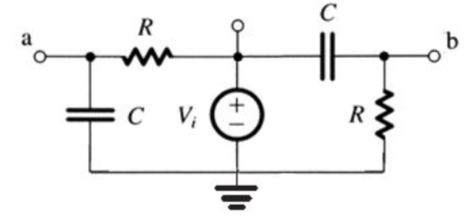
\includegraphics[height=3.2cm]{images/montagem.png}
\caption{Circuito com filtros passa alta e passa baixa}
\label{fig:montagem}
\end{figure}

\begin{figure}[h!]
\centering
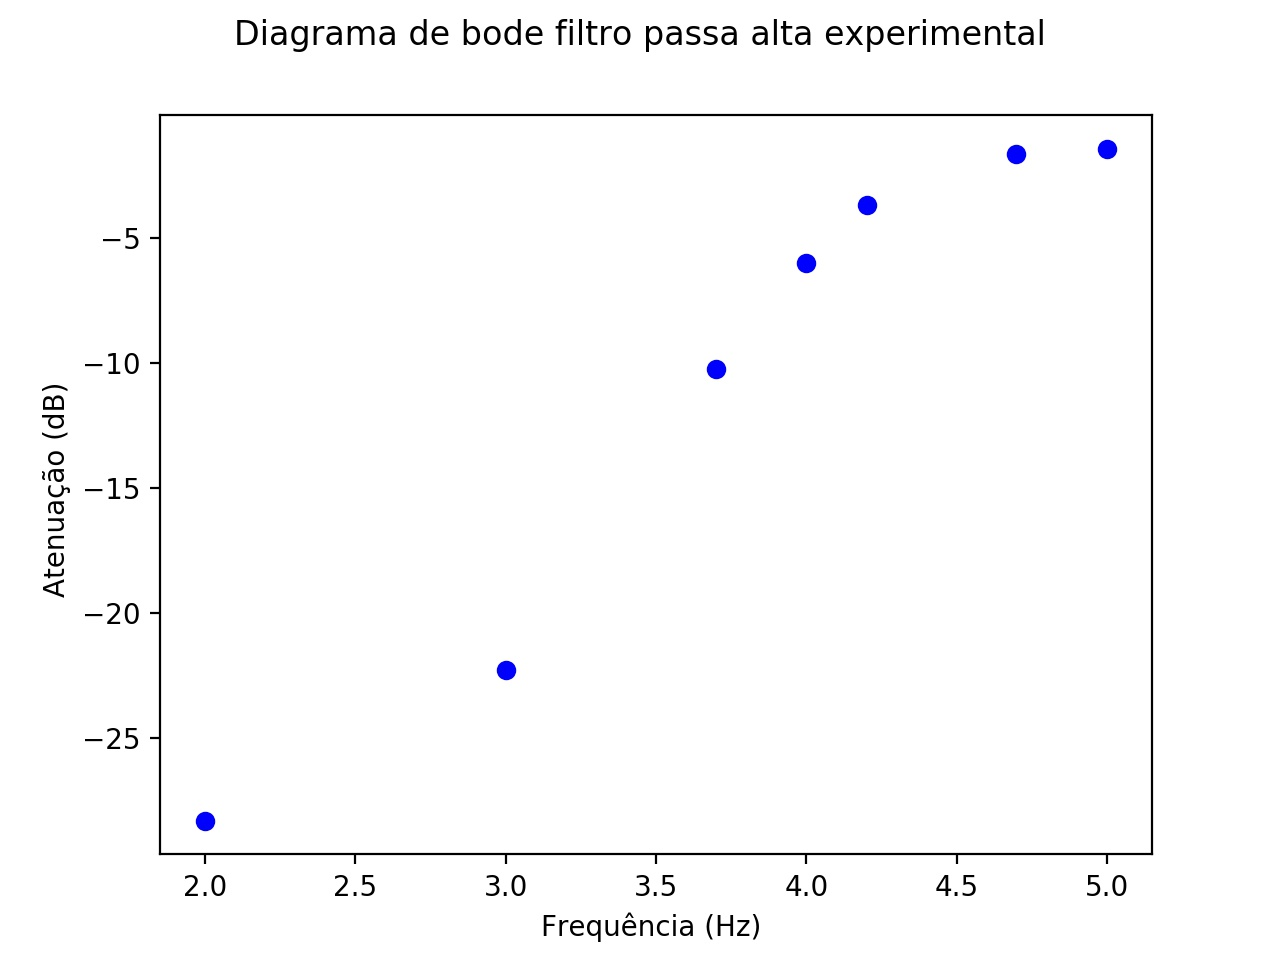
\includegraphics[height=8.2cm]{images/passa_alta_ate_exp.jpg}
\caption{Diagrama de bode para a atenuação do filtro passa alta}
\label{fig:passa_alta_atenuacao}
\end{figure}

\begin{figure}[h!]
\centering
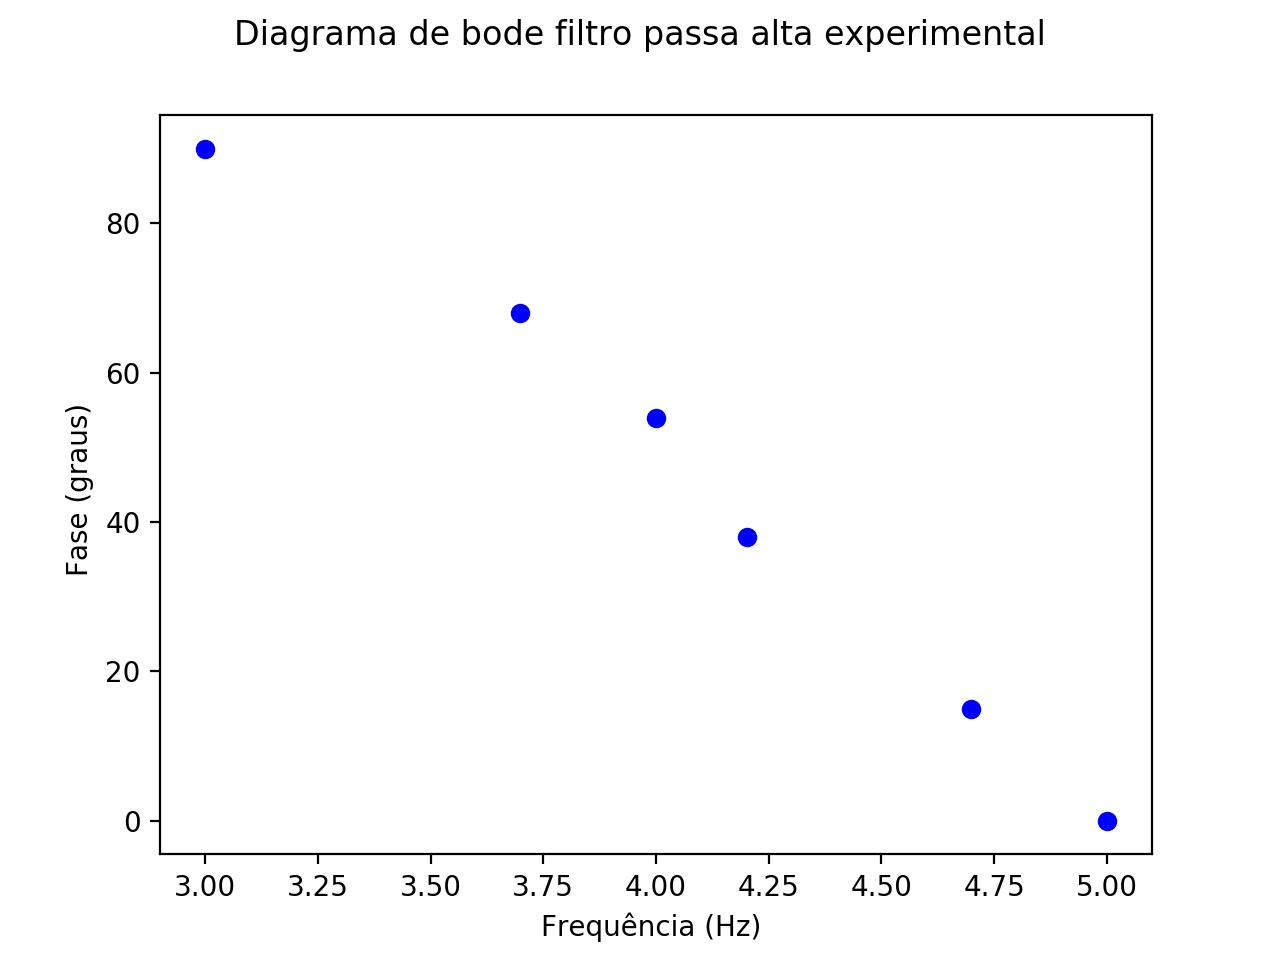
\includegraphics[height=8.2cm]{images/passa_alta_fase_exp.jpg}
\caption{Diagrama de bode para a fase do filtro passa alta}
\label{fig:passa_alta_fase}
\end{figure}

\begin{figure}[h!]
\centering
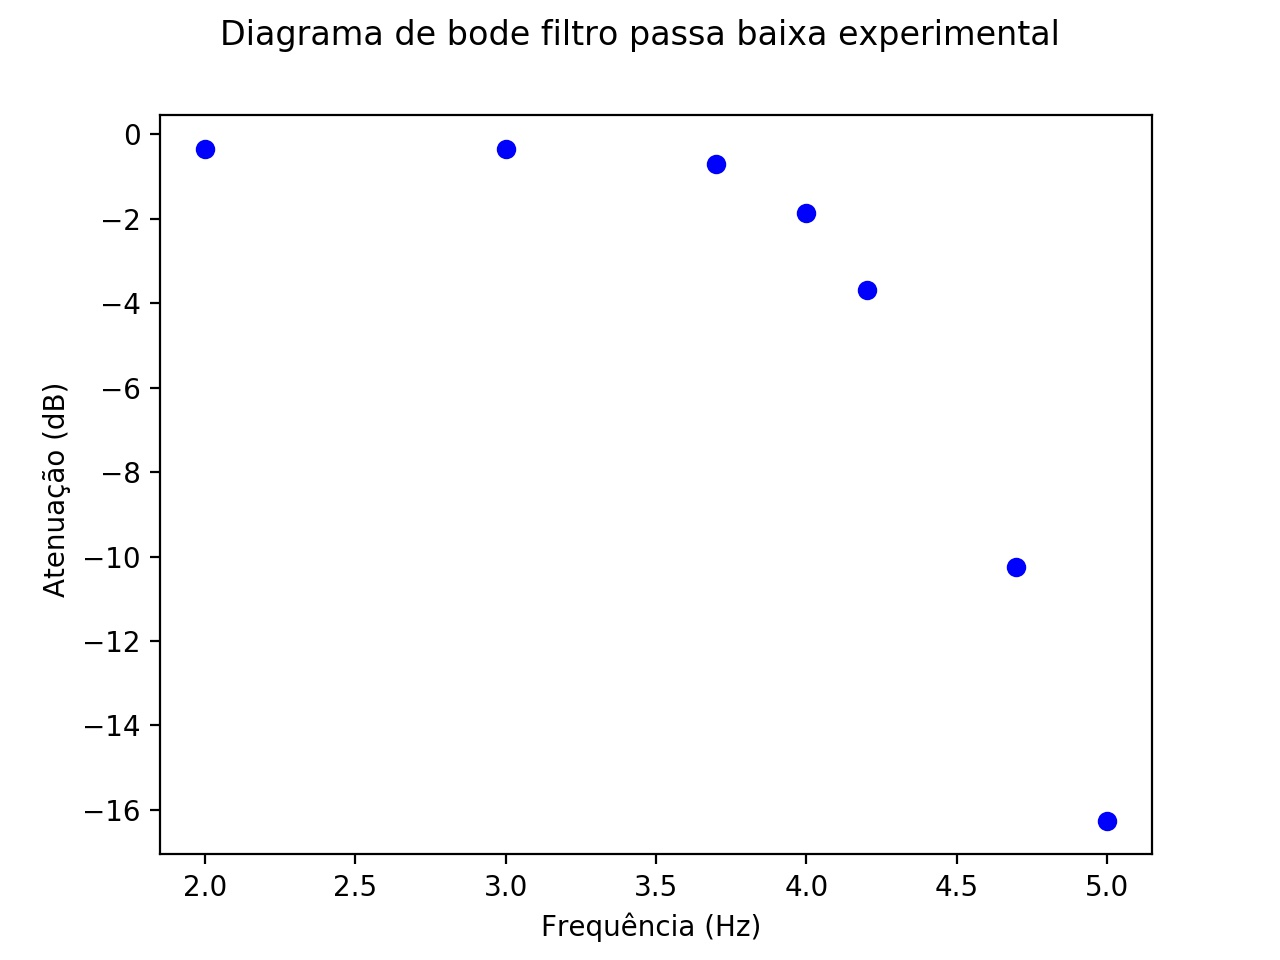
\includegraphics[height=8.2cm]{images/passa_baixa_ate_exp.jpg}
\caption{Diagrama de bode para a atenuação do filtro passa baixa}
\label{fig:passa_baixa_atenuacao}
\end{figure}

\begin{figure}[h!]
\centering
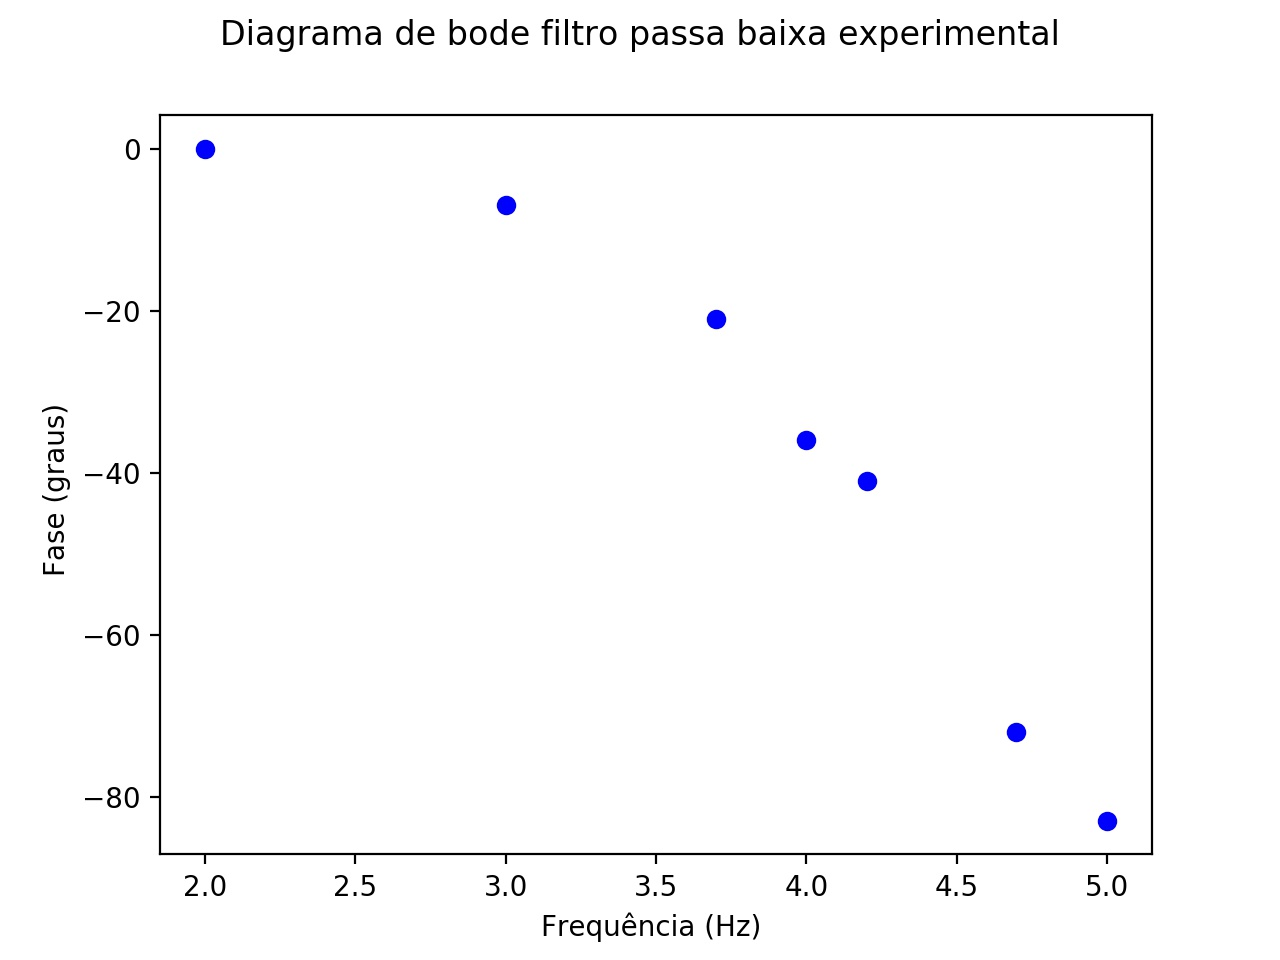
\includegraphics[height=8.2cm]{images/passa_baixa_fase_exp.jpg}
\caption{Diagrama de bode para a fase do filtro passa baixa}
\label{fig:passa_baixa_fase}
\end{figure}

\begin{figure}[h!]
\centering
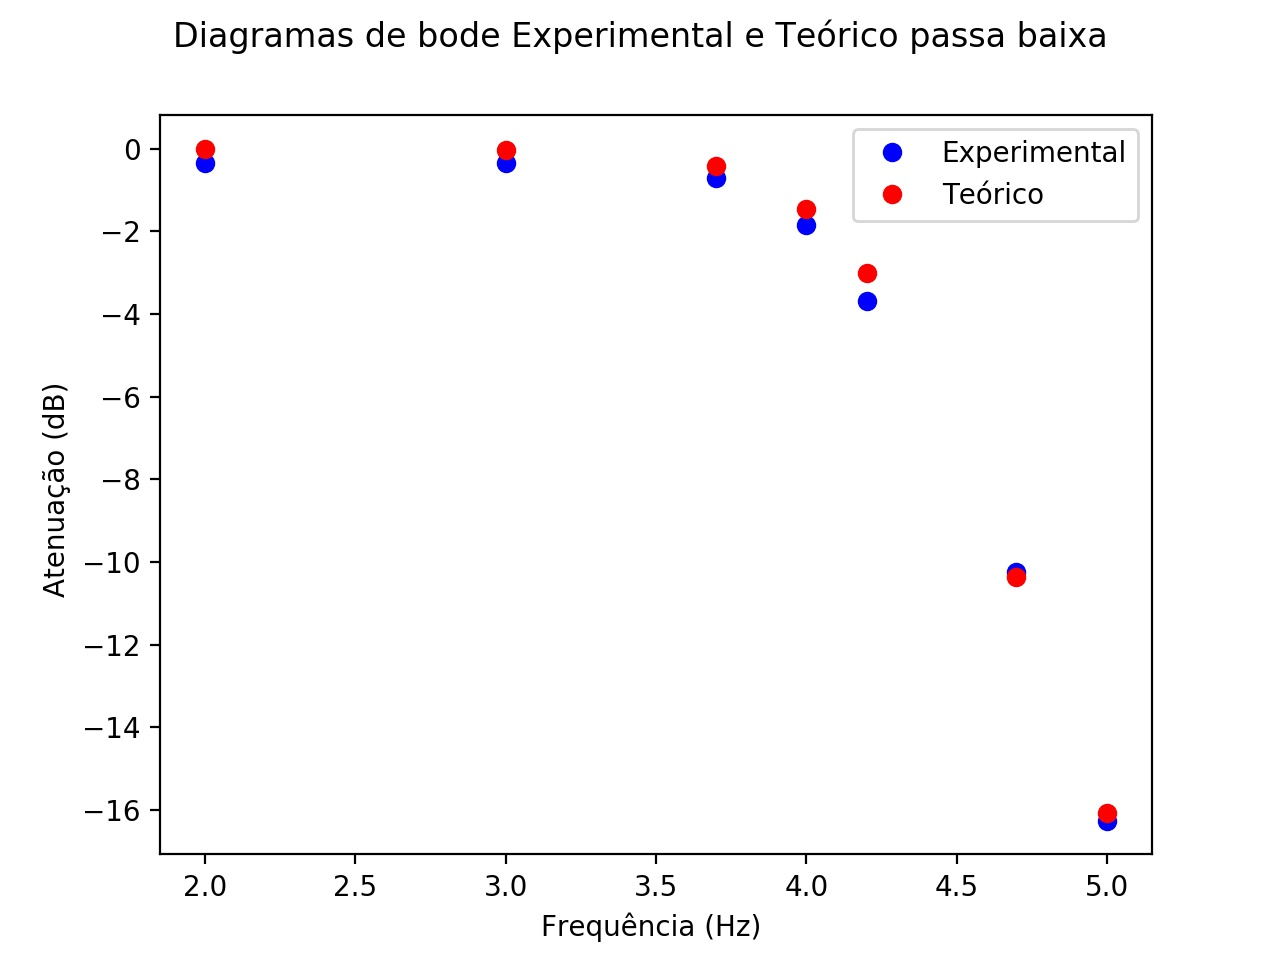
\includegraphics[height=8.2cm]{images/passa_baixa_ate_ambos.jpg}
\caption{Comparação dos diagramas teórico e experimental para a atenuação do filtro passa baixa}
\label{fig:passa_baixa_atenucao_ambos}
\end{figure}

\begin{figure}[h!]
\centering
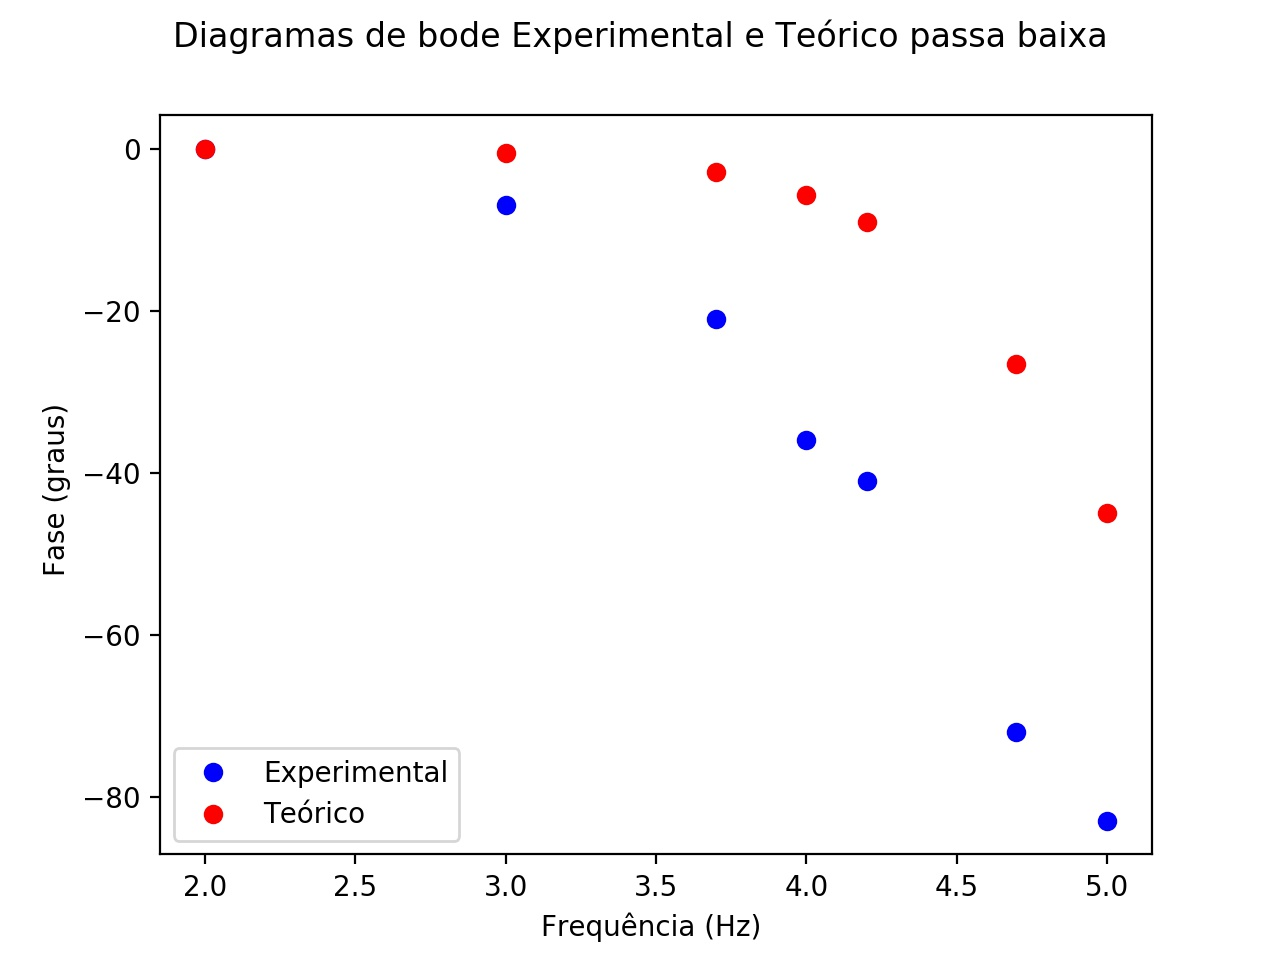
\includegraphics[height=8.2cm]{images/passa_baixa_fase_ambos.jpg}
\caption{Comparação dos diagramas teórico e experimental para a fase do filtro passa baixa}
\label{fig:passa_baixa_fase_ambos}
\end{figure}

\begin{figure}[h!]
\centering
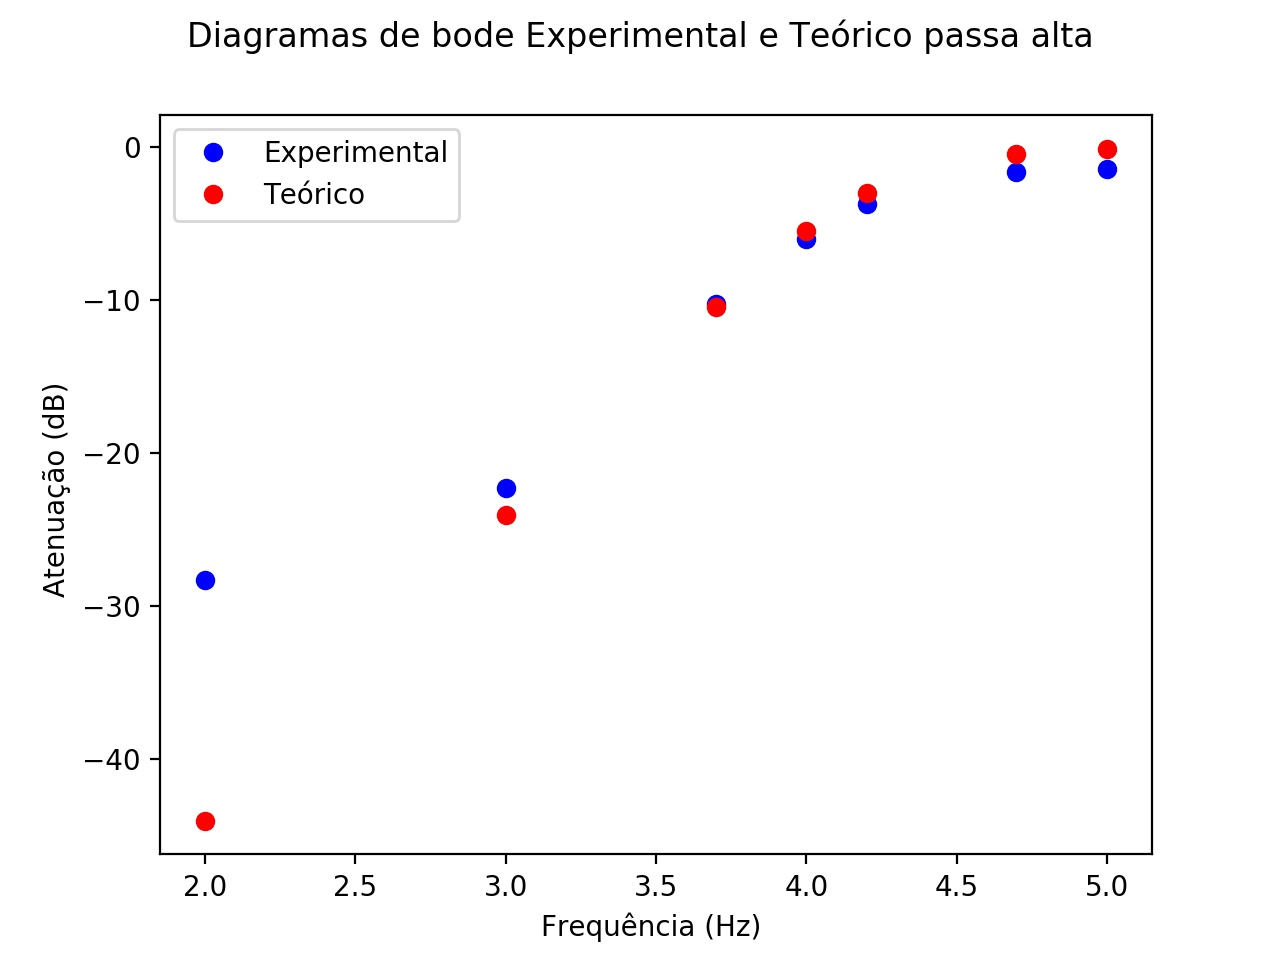
\includegraphics[height=8.2cm]{images/passa_alta_ate_ambos.jpg}
\caption{Comparação dos diagramas teórico e experimental para a atenuação do filtro passa alta}
\label{fig:passa_alta_atenucao_ambos}
\end{figure}

\begin{figure}[h!]
\centering
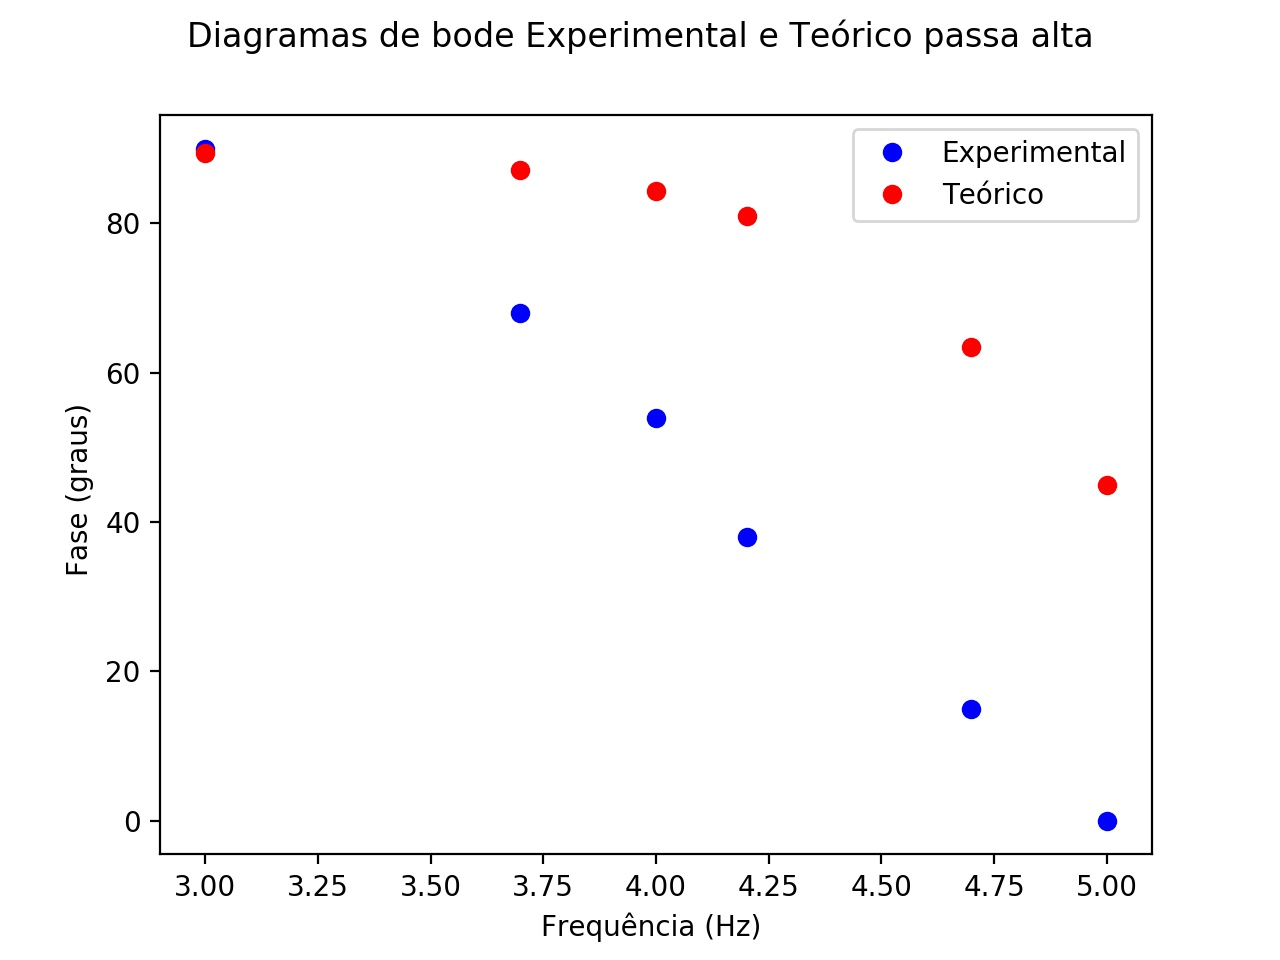
\includegraphics[height=8.2cm]{images/passa_alta_fase_ambos.jpg}
\caption{Comparação dos diagramas teórico e experimental para a fase do filtro passa alta}
\label{fig:passa_alta_fase_ambos}
\end{figure}


\begin{figure}[h!]
\centering
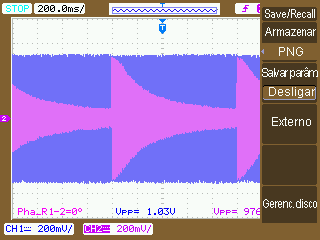
\includegraphics[height=6.2cm]{images/NewFile28.png}
\caption{Sweep para Filtro Passa Baixa}
\label{fig:sweep_baixa}
\end{figure}

\begin{figure}[h!]
\centering
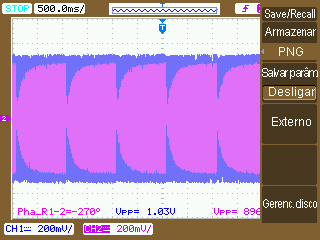
\includegraphics[height=6.2cm]{images/NewFile27.png}
\caption{Sweep para Filtro Passa Alta}
\label{fig:sweep_alta}
\end{figure}

\begin{table}[h!]
\caption{Dados experimentais obtidos para os filtros Passa Alta e Baixa}
\label{tabela:frequencias}
\begin{tabular}{|l|l|l|l|l|l|l|l|l|}
\hline
nó & Frequência & 100 & 1000 & 5000 & 10000 & 15915 & 50000 & 100000 \\ \hline
Vi & \begin{tabular}[c]{@{}l@{}}Amplitude\\ (pico a pico)\end{tabular} & 1.04 & 1.04 & 1.04 & 1.04 & 1.04 & 1.04 & 1.04 \\ \hline
\multicolumn{1}{|c|}{\multirow{3}{*}{\begin{tabular}[c]{@{}c@{}}Vo\\ {[}Passa baixa{]}\end{tabular}}} & \begin{tabular}[c]{@{}l@{}}Amplitude\\ (pico a pico)\end{tabular} & 1 & 1 & 0.96 & 0.84 & 0.68 & 0.32 & 0.16 \\ \cline{2-9} 
\multicolumn{1}{|c|}{} & \begin{tabular}[c]{@{}l@{}}Atenuação\\ (em dB)\end{tabular} & -0.341 & -0.341 & -0.695 & -1.855 & -3.690 & -10.238 & -16.258 \\ \cline{2-9} 
\multicolumn{1}{|c|}{} & \begin{tabular}[c]{@{}l@{}}Fase relativa\\ (a Vi)\end{tabular} & 0 & -7 & -21 & -36 & -41 & -72 & -83 \\ \hline
\multirow{3}{*}{\begin{tabular}[c]{@{}l@{}}Vo\\ {[}Passa alta{]}\end{tabular}} & \begin{tabular}[c]{@{}l@{}}Amplitude\\ (pico a pico)\end{tabular} & 0.04 & 0.08 & 0.32 & 0.52 & 0.68 & 0.86 & 0.88 \\ \cline{2-9} 
 & \begin{tabular}[c]{@{}l@{}}Atenuação\\ (em dB)\end{tabular} & -28.299 & -22.279 & -10.238 & -6.021 & -3.690 & -1.651 & -1.451 \\ \cline{2-9} 
 & \begin{tabular}[c]{@{}l@{}}Fase relativa\\ (a Vi)\end{tabular} & - & 90 & 68 & 54 & 38 & 15 & 0 \\ \hline
\end{tabular}
\end{table}

\end{document}
